\begin{figure}[!ht]
\centering

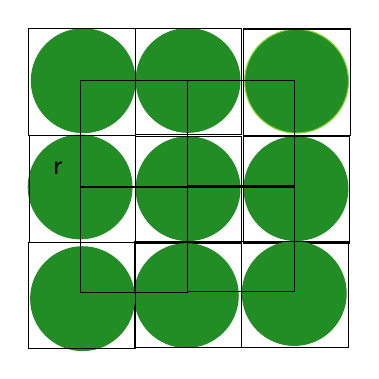
\begin{tikzpicture}[font=\sansmath\sffamily, x=0.75pt,y=0.75pt,yscale=-1,xscale=1]
%uncomment if require: \path (0,347); %set diagram left start at 0, and has height of 347

%Shape: Circle [id:dp09528747501265789] 
\draw  [color={rgb, 255:red, 34; green, 141; blue, 36 }  ,draw opacity=1 ][fill={rgb, 255:red, 34; green, 141; blue, 36 }  ,fill opacity=1 ] (337.33,165.33) .. controls (337.33,151.53) and (348.53,140.33) .. (362.33,140.33) .. controls (376.14,140.33) and (387.33,151.53) .. (387.33,165.33) .. controls (387.33,179.14) and (376.14,190.33) .. (362.33,190.33) .. controls (348.53,190.33) and (337.33,179.14) .. (337.33,165.33) -- cycle ;
%Shape: Square [id:dp5549834318221732] 
\draw   (336.93,140.2) -- (388.27,140.2) -- (388.27,191.53) -- (336.93,191.53) -- cycle ;
%Shape: Circle [id:dp254649691962442] 
\draw  [color={rgb, 255:red, 34; green, 141; blue, 36 }  ,draw opacity=1 ][fill={rgb, 255:red, 34; green, 141; blue, 36 }  ,fill opacity=1 ] (389.33,165.33) .. controls (389.33,151.53) and (400.53,140.33) .. (414.33,140.33) .. controls (428.14,140.33) and (439.33,151.53) .. (439.33,165.33) .. controls (439.33,179.14) and (428.14,190.33) .. (414.33,190.33) .. controls (400.53,190.33) and (389.33,179.14) .. (389.33,165.33) -- cycle ;
%Shape: Square [id:dp7521712816533537] 
\draw   (388.93,140.2) -- (440.27,140.2) -- (440.27,191.53) -- (388.93,191.53) -- cycle ;
%Shape: Circle [id:dp31352442918501755] 
\draw  [color={rgb, 255:red, 34; green, 141; blue, 36 }  ,draw opacity=1 ][fill={rgb, 255:red, 34; green, 141; blue, 36 }  ,fill opacity=1 ] (285.33,164.5) .. controls (285.33,150.69) and (296.53,139.5) .. (310.33,139.5) .. controls (324.14,139.5) and (335.33,150.69) .. (335.33,164.5) .. controls (335.33,178.31) and (324.14,189.5) .. (310.33,189.5) .. controls (296.53,189.5) and (285.33,178.31) .. (285.33,164.5) -- cycle ;
%Shape: Square [id:dp5215635546556922] 
\draw   (285.83,139.8) -- (337.17,139.8) -- (337.17,191.13) -- (285.83,191.13) -- cycle ;
%Shape: Circle [id:dp8519227919361114] 
\draw  [color={rgb, 255:red, 34; green, 141; blue, 36 }  ,draw opacity=1 ][fill={rgb, 255:red, 34; green, 141; blue, 36 }  ,fill opacity=1 ] (336.5,216.83) .. controls (336.5,203.03) and (347.69,191.83) .. (361.5,191.83) .. controls (375.31,191.83) and (386.5,203.03) .. (386.5,216.83) .. controls (386.5,230.64) and (375.31,241.83) .. (361.5,241.83) .. controls (347.69,241.83) and (336.5,230.64) .. (336.5,216.83) -- cycle ;
%Shape: Square [id:dp3236232559839335] 
\draw   (336.6,190.7) -- (387.93,190.7) -- (387.93,242.03) -- (336.6,242.03) -- cycle ;
%Shape: Circle [id:dp948966870385968] 
\draw  [color={rgb, 255:red, 34; green, 141; blue, 36 }  ,draw opacity=1 ][fill={rgb, 255:red, 34; green, 141; blue, 36 }  ,fill opacity=1 ] (337.33,113.17) .. controls (337.33,99.36) and (348.53,88.17) .. (362.33,88.17) .. controls (376.14,88.17) and (387.33,99.36) .. (387.33,113.17) .. controls (387.33,126.97) and (376.14,138.17) .. (362.33,138.17) .. controls (348.53,138.17) and (337.33,126.97) .. (337.33,113.17) -- cycle ;
%Shape: Square [id:dp7704640056265294] 
\draw   (336.93,88.03) -- (388.27,88.03) -- (388.27,139.37) -- (336.93,139.37) -- cycle ;
%Shape: Circle [id:dp21750961656288648] 
\draw  [color={rgb, 255:red, 34; green, 141; blue, 36 }  ,draw opacity=1 ][fill={rgb, 255:red, 34; green, 141; blue, 36 }  ,fill opacity=1 ] (286.83,113.33) .. controls (286.83,99.53) and (298.03,88.33) .. (311.83,88.33) .. controls (325.64,88.33) and (336.83,99.53) .. (336.83,113.33) .. controls (336.83,127.14) and (325.64,138.33) .. (311.83,138.33) .. controls (298.03,138.33) and (286.83,127.14) .. (286.83,113.33) -- cycle ;
%Shape: Square [id:dp023375777050106628] 
\draw   (285.53,88.2) -- (336.87,88.2) -- (336.87,139.53) -- (285.53,139.53) -- cycle ;
%Shape: Circle [id:dp08410780423004927] 
\draw  [color={rgb, 255:red, 126; green, 211; blue, 33 }  ,draw opacity=1 ][fill={rgb, 255:red, 34; green, 141; blue, 36 }  ,fill opacity=1 ] (389.63,113.53) .. controls (389.63,99.73) and (400.83,88.53) .. (414.63,88.53) .. controls (428.44,88.53) and (439.63,99.73) .. (439.63,113.53) .. controls (439.63,127.34) and (428.44,138.53) .. (414.63,138.53) .. controls (400.83,138.53) and (389.63,127.34) .. (389.63,113.53) -- cycle ;
%Shape: Square [id:dp4096382997581849] 
\draw   (389.23,88.4) -- (440.57,88.4) -- (440.57,139.73) -- (389.23,139.73) -- cycle ;
%Shape: Circle [id:dp2759735468682599] 
\draw  [color={rgb, 255:red, 34; green, 141; blue, 36 }  ,draw opacity=1 ][fill={rgb, 255:red, 34; green, 141; blue, 36 }  ,fill opacity=1 ] (286.5,218.33) .. controls (286.5,204.53) and (297.69,193.33) .. (311.5,193.33) .. controls (325.31,193.33) and (336.5,204.53) .. (336.5,218.33) .. controls (336.5,232.14) and (325.31,243.33) .. (311.5,243.33) .. controls (297.69,243.33) and (286.5,232.14) .. (286.5,218.33) -- cycle ;
%Shape: Square [id:dp8215492752117758] 
\draw   (285.6,191.2) -- (336.93,191.2) -- (336.93,242.53) -- (285.6,242.53) -- cycle ;
%Shape: Circle [id:dp09537557723600643] 
\draw  [color={rgb, 255:red, 34; green, 141; blue, 36 }  ,draw opacity=1 ][fill={rgb, 255:red, 34; green, 141; blue, 36 }  ,fill opacity=1 ] (388.5,215.83) .. controls (388.5,202.03) and (399.69,190.83) .. (413.5,190.83) .. controls (427.31,190.83) and (438.5,202.03) .. (438.5,215.83) .. controls (438.5,229.64) and (427.31,240.83) .. (413.5,240.83) .. controls (399.69,240.83) and (388.5,229.64) .. (388.5,215.83) -- cycle ;
%Shape: Square [id:dp6889139441622811] 
\draw   (388.1,190.7) -- (439.43,190.7) -- (439.43,242.03) -- (388.1,242.03) -- cycle ;
%Shape: Square [id:dp8182120104489065] 
\draw   (310.6,113.2) -- (361.93,113.2) -- (361.93,164.53) -- (310.6,164.53) -- cycle ;
%Shape: Square [id:dp9870127822168651] 
\draw   (362.1,113.2) -- (413.43,113.2) -- (413.43,164.53) -- (362.1,164.53) -- cycle ;
%Shape: Square [id:dp4726375642600965] 
\draw   (310.6,164.2) -- (361.93,164.2) -- (361.93,215.53) -- (310.6,215.53) -- cycle ;
%Shape: Square [id:dp991370682204621] 
\draw   (362.1,163.7) -- (413.43,163.7) -- (413.43,215.03) -- (362.1,215.03) -- cycle ;

% Text Node
\draw (303.16,155.64) node   [align=left] {\begin{minipage}[lt]{8.67pt}\setlength\topsep{0pt}
r
\end{minipage}};


\end{tikzpicture}

\caption{Mặt cắt ngang của một phần trong mạng tinh thể}
\label{P2_tikz2}
\end{figure}

